% ********** Material Chapter **********
\chapter{The Properties of Doped and Strained Silicon} 
\label{cha:material}
\epigraph{`Without electrons, there is no Google.'}{\mbox{\textup{---\textsc{Jeff Goodell}}}}
%
\section{Introduction}\label{sec:material-introduction}
The work detailed in this thesis explains the development (and hoped improvement) of the already existing cold-electron bolometer by replacing the normal-metal absorbing element used in previous devices \parencite{Kuzmin2004,Otto2013} with highly-doped strained silicon. As such, it is useful to address the underlying principle of semiconductors and how their characteristics can be altered by either doping the material or by straining the material's atomic lattice.% While this chapter will cover the principles directly relevant to \glspl{gls:CEB} a much more complete description of the field of semiconductors can be found in \citetitle{Kittel2005} by \textcite{Kittel2005}.

\section{Intrinsic Semiconductors}\label{sec:intrinsic-semiconductors}
As is implied by their name, semiconductors are materials which are partially conductive---that is to say, they do not conduct in the same way as a metal but nor do they prevent all current flow, as insulators do. Semiconductors have a crystal lattice of atoms; the formation of this lattice can result in the creation of \textit{free} electrons, these free electrons cease to be tightly bound to their parent nuclei (they are referred to as \textit{delocalised}) and can flow (as current) through the crystal lattice of the material. In order for a \textit{delocalised} electron to be able to flow as a current through the material, it must first be removed from the atom to which it belongs by gaining a certain amount of energy (depending upon how tightly bound it is to the atom). This energy can be in the form of thermal energy from heating the crystal (as such semiconductors, unlike metals, have an electrical conductivity which increases with temperature) or by providing an external electrical bias across the material.
\begin{figure}[t]
\begin{center}
\includegraphics[width = 0.5\textwidth]{figures/Semiconductor_intrinsic}
\caption[Band structure of an intrinsic semiconductor]{Band structure of an intrinsic semiconductor. With no additional energy for the electrons to absorb, all the electrons are bound to their nucleus and exist in the valence band. In order to flow as a current, they must gain enough energy to break their binding to the nucleus. For the most weakly bound electrons, this energy corresponds to the band gap energy, $E_{\mathrm{g}}$. $E_{\mathrm{f}}$ is the Fermi level, for an intrinsic (undoped) semiconductor, this is located halfway through the energy gap.}
\label{fig:intrinsicSemiconductorBands}
\end{center}
\end{figure}
\par 
The requirement for an energy threshold to be gained before an electron can flow as current can be thought of in terms of a energy band diagram, as shown in Figure~\ref{fig:intrinsicSemiconductorBands}. Without the input of any additional energy, all the electrons are bound to their respective nuclei and are unable to flow as current through the material (the material is an insulator). These electrons have low energies and exist in the valence band shown in Figure~\ref{fig:intrinsicSemiconductorBands}. The top of the valence band corresponds to the energy level of the most weakly bound electrons (that is the energy level of the outer most electron shell). However, this does not mean that any infinitely small increase in the energy of these electrons will liberate them from their nuclei, instead they must gain enough energy to enter the conduction band. This means that, for the electrons in the outermost electron shells to be able to flow as current, they must gain enough energy to \textit{jump} through the band gap; this is the band gap energy and has a value of $E_{\mathrm{g}}$.\footnote{Throughout this work $E_{\mathrm{g}}$ will be used to refer to the band gap energy of a semiconductor to avoid confusion with $\varDelta$, which is used to denote half of the energy gap in a superconductor.}

\section{Doped Semiconductors}\label{sec:doped-semiconductors}
The intrinsic semiconductor, explained above and whose energy level diagram is shown in Figure~\ref{fig:intrinsicSemiconductorBands}, is the basis for all forms of semiconductors and can be thought of as being characterised (at least in the sense of its energy distribution) by the size of its energy gap. However, one key advantage of semiconductors is that their conductivity can be controlled by adding impurities to the crystal lattice, this process is called \textit{doping}.
\begin{figure}[t]
\begin{center}
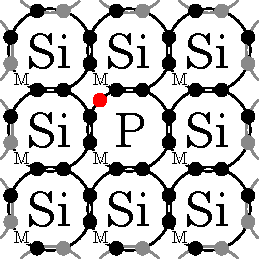
\includegraphics[width = 0.4\textwidth]{figures/n_type_doping}
\caption[Crystal lattice of silicon with an n-type dopant inserted.]{Crystal lattice of silicon with an n-type dopant (phosphorus in this case) grown into the lattice. For n-type doping, the dopant has more electrons in its outer shell than are required to form covalent bonds with the surrounding atoms in the lattice, this results in an additional electron (highlighted in red above) which is not bound to the crystal lattice and acts as a \textit{free} electron, increasing conductivity.}
\label{fig:nTypeDoing}
\end{center}
\end{figure}
\par
In order for the doping to alter the electrical characteristics of a semiconductor, the impurity added must bond to the crystal lattice in such a way that an unbound electron is added to the crystal or that a vacant electron state is created. Figure~\ref{fig:nTypeDoing} illustrates the case where an unbound electron is added (refereed to as \textit{n-type} doping, since a negative charge is added to the crystal). In this case, the dopant impurity (phosphors in Figure~\ref{fig:nTypeDoing}) has five electrons in its outer shell; four of these form covalent bonds with neighboring silicon atoms, however, one electron does not form a covalent bond. The impurity is called a \textit{donor} since, when ionised by sufficient energy, the atom \textit{donates} an electron to the conduction band, this has the net effect of increasing the conductivity of the semiconductor.
\begin{figure}[t]
\begin{center}
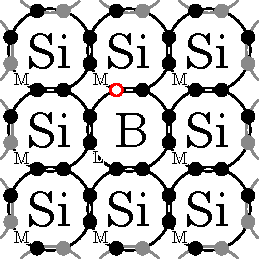
\includegraphics[width = 0.4\textwidth]{figures/p_type_doping}
\caption[Crystal lattice of silicon with a p-type dopant inserted.]{Crystal lattice of silicon with a p-type dopant (boron) grown into the lattice. For p-type doping, the dopant has fewer electrons in its outer shell than the neighboring atoms. This means the atom does not form covalent bonds with all of the neighboring atoms and a hole (highlighted red) is created.}
\label{fig:pTypeDoing}
\end{center}
\end{figure}
\par
The opposite of n-type doping is \textit{p-type} doping (the `p' denotes positive charge), where the dopant used has fewer electrons in its outer electron shell than the rest of the atoms in the lattice. This means that there are incomplete covalent bonds (or \textit{holes}) in the crystal structure, which can capture free electrons. This is illustrated in Figure~\ref{fig:pTypeDoing}, where boron has been grown into a lattice of silicon. Boron is a group \Rom{13} element and has three electrons in its outer shell, compared to silicon which has four (group \Rom{14}); this \textit{missing} electron (shown in Figure~\ref{fig:pTypeDoing} as an empty red circle) means that a covalent bond is unable to form between the dopant and one of the neighboring silicon atoms. The dopant in this case is referred to as an \textit{acceptor}, since an electron can become bound or \textit{accepted} into the vacant state. Like n-type doping, p-type doping also has the effect of increasing the conductivity since, when ionised, the hole can become mobile and move through the lattice meaning that electrons switch places with the hole and thus also move through the lattice.
\begin{figure}[t]
\begin{center}
\subfloat[]{
	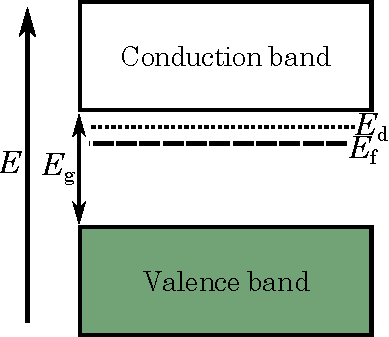
\includegraphics[height=0.2\textheight]{figures/n_type_energyLevels}
	\label{fig:n-type_enrgyLevels}
}
\hspace{0.00\textwidth}
\subfloat[]{
	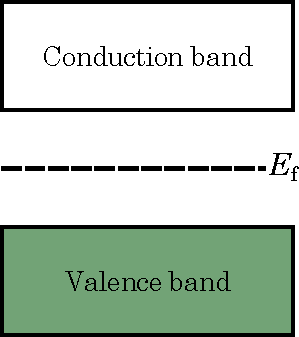
\includegraphics[height=0.2\textheight]{figures/intrinsic_energyLevels}
	\label{fig:intrinsic_enegyLevels}
}
\hspace{0.00\textwidth}
\subfloat[]{
	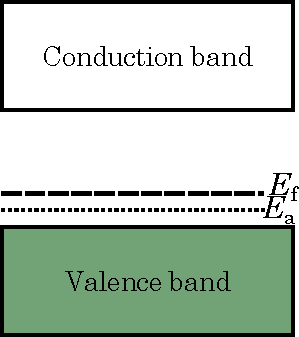
\includegraphics[height=0.2\textheight]{figures/p_type_energyLevels}
	\label{fig:p-type_enrgyLevels}
}
\caption[Energy level diagrams for doped semiconductors]{Energy level diagrams for doped semiconductor. (a) N-type doped semiconductor---since the dopant adds an additional electron to the lattice, the Fermi energy ($E_{\mathrm{f}}$) is increased; $E_{\mathrm{d}}$ is the ionisation energy required to unbind the additional electron of the donor dopant from its parent nucleus. (b) Intrinsic semiconductor---since there are no dopants present in the lattice, there are no ionisation levels and the Fermi energy is in the middle of the band gap (as was seen in Figure~\ref{fig:intrinsicSemiconductorBands}). (c) P-type doped semiconductor---the dopant reduces the number of electrons (compared to an intrinsic semiconductor) and thus the Fermi energy is reduced; $E_{\mathrm{a}}$ is the ionisation energy required to unbind the hole state from the acceptor dopant.}
\label{fig:dopingEnergyLevels}
\end{center}
\end{figure}
\par 
Since doping alters the distribution of electrons in a semiconductor, the energy level diagrams for doped semiconductors differ from that of an intrinsic semiconductor (shown in Figure~\ref{fig:intrinsicSemiconductorBands}). Figure~\ref{fig:dopingEnergyLevels} shows the energy level diagrams for n- and p-type semiconductors (Figures~\ref{fig:n-type_enrgyLevels} and \ref{fig:p-type_enrgyLevels}), along with that of an intrinsic semiconductor (Figure~\ref{fig:intrinsic_enegyLevels}), for comparison. For doped semiconductors, the energy level diagram includes an additional level corresponding to the ionisation energy of either the additional electron from the donor atom (n-type), $E_{\mathrm{d}}$, or hole state from the acceptor atom (p-type), $E_{\mathrm{a}}$. Since n-type doping creates a positively charged region (due to the addition of one or more electrons), the Fermi energy in an n-type semiconductor is increased (moved towards the conduction band) compared to the intrinsic case (Figure~\ref{fig:intrinsic_enegyLevels}). In the case of p-type doping, the dopant creates a positively charged region around it, where there is a shortage of electrons; this has the effect of decreasing the Fermi energy in comparison to the intrinsic case.
\par 
One important physical feature of doping worth mentioning is that, since the dopant is added to the lattice during its growth, it does not displace an atom but instead simply forms as part of the lattice.
\par 
By increasing the number of dopants present within the lattice, the degree by which the conductivity of the lattice is altered can be carefully controlled. \textcite{Pearson1949} showed that introducing phosphorus dopants to a silicon lattice (n-type doping) at a concentration of $4.7 \times 10^{17}~\mathrm{cm^{-3}}$ resulted in decreasing the materials resistivity to $0.3~\mathrm{\Omega\,cm}$ at room temperature, compared to $\approx 10^{6}~\mathrm{\Omega\,cm}$ in the absence of any dopant atoms. Furthermore, increasing the doping concentration further to $4.7 \times 10^{20}~\mathrm{cm^{-3}}$ (equivalent to approximately one per cent phosphorus) resulted in a resistivity of $7 \times 10^{-4}~\mathrm{\Omega\,cm}$.
\par 
The terminology of doped semiconductors typically distinguishes four vague levels of doping: \textit{lightly-doped} semiconductors have doping levels  $\lessapprox 10^{14}~\mathrm{cm^{-3}}$; this can be written as \textit{n\textsuperscript{$-$}-} or \textit{p\textsuperscript{$-$}-type} doping; \textit{moderately-doped} semiconductors have dopant concentrations in the range $10^{14}\mbox{--}10^{16}~\mathrm{cm^{-3}}$; \textit{heavily-doped} is typically used in relation to doping levels in the approximate range $10^{16}\mbox{--}10^{18}~\mathrm{cm^{-3}}$ and this level of doping is often expressed as \textit{n\textsuperscript{+}-} or \textit{p\textsuperscript{+}-type} doping; finally, when the doping level is such that the electrical behaviour of the material can be thought of as being analogous to a metal, it is referred to as being \textit{degenerate}, this typically involves doping levels $> 10^{18}~\mathrm{cm^{-3}}$ and is written as \textit{n\textsuperscript{++}-} or \textit{p\textsuperscript{++}-type} doping. While---as is true in various areas of physics---there are no exact guidelines or boundaries as to when a material ceases to be classed as lightly-doped and becomes moderately-doped, the term degenerate should be reserved in use for semiconductors which are doped to a sufficient level that they behave (electrically) like a metal.
%
\section{Carrier Mobility}\label{sec:material-mobility}
The \textit{mobility} of an electron or hole in a semiconducting crystal is defined as the speed at which the charge carrier \textit{drifts} through the lattice per unit electric field. As such, the mobility, $\mu$, is defined by:
\begin{align}
\mu &= \frac{\left|v\right|}{E}\,, \label{eqn:mobility}
\end{align} 
where $\left|v\right|$ is the modulus of the carrier's drift velocity and $E$ is the electric field to which the carrier is subjected. The modulus of the drift velocity is used since mobility of electrons and holes ($\mu_{\mathrm{e}}$ and $\mu_{\mathrm{h}}$ respectively) are both defined to be positive, despite the fact that for an applied field of given polarity, the two carrier types will move or drift in opposite directions.
\par 
It is easy to understand the relationship between the carrier mobility and the doping concentration by considering the movement of the carriers through the lattice. When an electric field is applied, the carrier will be accelerated by the field; if the carrier were moving through free space, then, due to the acceleration, its velocity would continue to increase to approaching the speed of light. However, in the crystal structure, the carrier frequently collides with other particles (such as defects or impurities in the lattice), this causes the velocity of the carrier (on scales larger than the mean free path between collisions) to be limited to some equilibrium between the accelerating force from the electric field and rate of collisions experienced. This velocity is the drift velocity referred to in Equation~\ref{eqn:mobility}. After activation, each dopant atom added to the lattice becomes ionised; as the carriers move through the lattice, they collide with these ions and this decreases their drift velocity (and thus their mobility). Clearly, increasing the doping concentration (and thus the number of ions) increases the frequency of collisions experienced by the carriers and accordingly their drift velocity and thus their mobility is decreased.
\par 
Data showing the overall relation between the mobility and the doping concentration, for both electrons and holes, was compiled by \textcite{Caughey1967}\footnote{There is a mistake in \citeauthor{Caughey1967}'s manuscript, the captions of Figures 1 and 2 should be switched.} who, in turn, drew heavily on the data of \textcite{Irvin1962}. \citeauthor{Caughey1967} used simple curve fitting techniques to fit the collected data. They showed that, to a reasonable level, the data for both the mobility of electrons and holes could be fitted by:
\begin{align}
\mu &= \frac{\mu_{\mathrm{max}} - \mu_{\mathrm{min}}}{1 + \left(\frac{N}{N_{\mathrm{ref}}}\right)^{\alpha}} + \mu_{\mathrm{min}}\,,
	\label{eqn:mobilityFit}
\end{align}
where $N$ is the number of dopant atoms per cubic centimetre, $\mu_{\mathrm{max}}$ and $\mu_{\mathrm{min}}$ are the maximum and minimum measured mobilities, $N_{\mathrm{ref}}$ is the total number of atoms per cubic centimetre, and $\alpha$ is a curve-fitting constant. All of these terms are dependent not only on the material but also on the carrier being studied. The fitting parameters found by \textcite{Caughey1967} are given in Table~\ref{tab:mobilityFitting} and their graph showing the fit to data collected for electron mobilities is reproduced in Figure~\ref{fig:electronMobilityDoping}
\begin{table}[htb]
\caption{Carrier mobility curve-fitting parameters from \textcite{Caughey1967}.} 
\label{tab:mobilityFitting}
\centering
\begin{tabular}{lS[table-format=4.0]
S[table-format=2.1]S[table-format=1.2]c}
\toprule\toprule
{Carrier} & {$\mu_{\mathrm{max}}~\left(\mathrm{cm^{2}\,V^{-1}\,s^{-1}}\right)$} &
{$\mu_{\mathrm{min}}~\left(\mathrm{cm^{2}\,V^{-1}\,s^{-1}}\right)$} & {$\alpha$} & 
{$N_{\mathrm{ref}}~\left(\mathrm{cm^{-3}}\right)$}\\ \midrule
Holes & 495 & 47.7 & 0.76 & $6.3\times 10^{16}$ \\
Electrons & 1330 & 65 & 0.72 & $8.5\times 10^{16}$ \\ \bottomrule
\end{tabular}
\end{table}
\begin{figure}[t]
\begin{center}
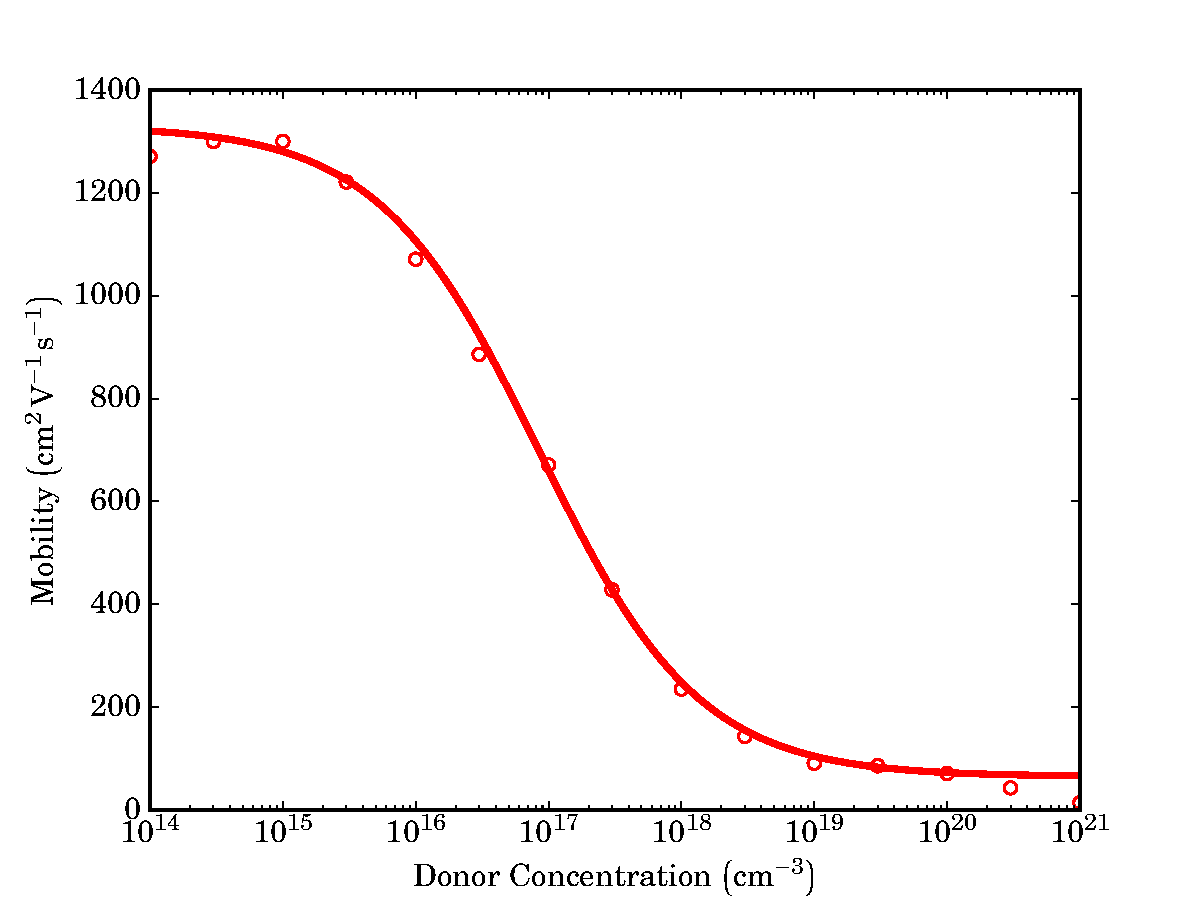
\includegraphics[width = 0.95\textwidth]{figures/CaugheyData}
\caption[Change in electron mobility with increasing donor concentration]{Decrease in electron mobility with increasing donor concentration. Circles---data, solid line---model fit. Reproduced, with permission, from \textcite{Caughey1967}. \copyright 1967 IEEE.}
\label{fig:electronMobilityDoping}
\end{center}
\end{figure}
\par 
While Equation~\ref{eqn:mobilityFit}, along with the parameters found by \textcite{Caughey1967}, do not produce a complete model of the mobility based on physical processes, they do act as a relatively accurate means of predicting the carrier mobility for a particular value of doping concentration.
%
\section{Strained Semiconductors} \label{sec:material-strain}
Straining silicon is the process of forcing the silicon atoms in the lattice to be slightly further apart than they would be naturally (the interatomic spacing is increased). This is achieved by growing silicon atop a buffer layer consisting of a material which has a larger atomic spacing than that of the silicon. Silicon germanium is commonly used as the buffer or straining layer, since it readily forms bonds to the silicon lattice, also the lattice spacing of this layer---and thus the level of strain in the silicon---can be controlled by adjusting the ratio of germanium in the silicon germanium. The concept behind the introduction of strain to a silicon lattice is shown in Figure~\ref{fig:strainFormation}.
\begin{figure}[t]
\begin{center}
\subfloat[]{
	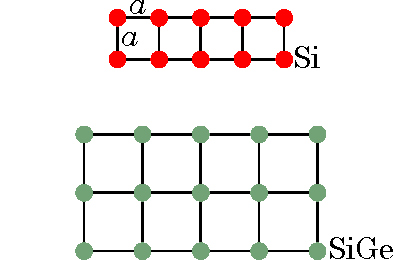
\includegraphics[width=0.5\textwidth]{figures/StrainFormation_before}
	\label{fig:strainFormation_before}
}
\subfloat[]{
	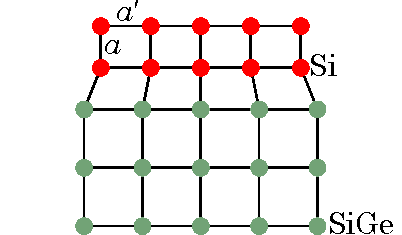
\includegraphics[width=0.5\textwidth]{figures/StrainFormation_after}
	\label{fig:strainFormation_after}
}
\caption[Introducing strain into a silicon lattice]{Introducing strain into a silicon lattice. (a) Silicon and silicon germanium as isolated lattices; the two materials have independent lattice spacings and, in both cases, the lattice spacing in both directions are the same, which is equal to $a$ for the silicon lattice (a simple two-dimensional model is shown). (b) The effect of growing silicon atop a layer of silicon germanium; the lattice becomes stretched or strained in the plane of the silicon germanium layer, changing the lattice spacing in this plane to $a'$ while the lattice spacing in the vertical direction is unchanged.}
\label{fig:strainFormation}
\end{center}
\end{figure}
\par 
The most common reason to introduce strain into a silicon lattice is to increase the carrier mobility. This occurs due to the strain forces stretching the crystal lattice, increasing the interatomic spacing and thus increasing the mean free path length between scattering events for the carriers. This is highly advantageous in the field of semiconducting electronic components where, for example, strained silicon offers substantial increases to the switching speed of transistors, allowing for faster microprocessors. The improvement in carrier mobilities was first demonstrated by \textcite{Welser1994}, who showed that at low applied electric fields, the electron mobility in n-doped ($N \approx 2 \times 10^{15}~\mathrm{cm^{-3}}$) silicon, strained by a SiGe layer (Si\textsubscript{0.7}Ge\textsubscript{0.3}), was increased to $\approx 1600~\mathrm{cm^{2}\,V^{-1}\,s^{-1}}$ compared to $\approx 600~\mathrm{cm^{2}\,V^{-1}\,s^{-1}}$ for a comparable unstrained system.
\par 
Another reason (particularly relevant to the field of detectors) to introduce strain into the silicon is that strained silicon has been shown by \textcite{Muhonen2011} to offer decreased coupling between the electrons and the phonons. \citeauthor{Muhonen2011} showed that at sub-Kelvin temperatures, the heat flow between the electrons and the phonons was reduced by a factor of between 20--50, depending on the lattice temperature. In terms of detector performance, this decrease in the electron-phonon coupling can increase a detector's sensitivity by decreasing the heat flow noise (from Equation~\ref{eqn:e-phNoise}). Furthermore, since the electrons are more thermally isolated from the lattice phonons they can, when cooled as described in Sections~\ref{sec:theory-current} and \ref{sec:theory-power}, be cooled further below the lattice temperature compared to electrons in an unstrained material. This was shown by \textcite{Prest2011}, who used the same material described by \textcite{Muhonen2011} as the central island of a microrefrigerator device. \citeauthor{Prest2011} showed that, at a lattice temperature of $300~\mathrm{mK}$, a device utilising strained silicon was capable of cooling electrons to a minimum temperature of $174~\mathrm{mK}$, compared to $258~\mathrm{mK}$ for a device using unstrained silicon. This increase in performance is directly applicable to the cold-electron bolometer, not only in decreasing the heat flow noise, but also by allowing the electrons in the absorber to operate at lower temperatures, reducing the majority of noise contributions detailed in Section~\ref{sec:theory-noise}.
%\reminder{Optical Properties and modelling (FP model).}
